En este capitulo se detallan los objetivos, la metodología que se utiliza, y las tecnologías en la cual se apoya.

\section{Objetivos del proyecto}

\subsection{Objetivo General}
Desarrollar una aplicación en Unity que permita simular el laboratorio
del CIMUBB, con la cual los estudiantes puedan probar el funcionamiento de los
brazos robóticos SCORBOT ER V Plus y el brazo robótico SCORBOT ER IX , intentando replicar con el mayor detalle posible
las estaciones de los brazos en el laboratorio.

\subsection{Objetivos Específicos}
\begin{enumerate}[label=\roman*.-]
\item Examinar los desafíos inherentes de la problemática que presenta el laboratorio, para establecer una base solida y asegurar la efectividad del software.
\item Analizar tecnologías y herramientas con el fin de comprender su funcionamiento y utilizarlas de manera eficaz en la resolución del problema.
\item Iniciar el desarrollo de la aplicación para proporcionar el software del proyecto.
\end{enumerate}

\subsection{Actividades}
Las actividades desarrolladas en este proyecto son:
\begin{enumerate}[label=\roman*.-]
\item Examinar los desafíos inherentes de la problemática que presenta el laboratorio, para establecer una base solida y asegurar la efectividad del software.
    \begin{enumerate}[label=\arabic*.-]
    \item Investigación sobre los factores que originan la problemática.
    \end{enumerate}
\item Analizar tecnologías y herramientas con el fin de comprender su funcionamiento y utilizarlas de manera eficaz en la resolución del problema.
    \begin{enumerate}[label=\arabic*.-]
    \item Exploración y análisis de diversas herramientas de programación con el propósito de comprender sus características y funcionalidades.
    \item Investigación para evaluar las posibilidades que ofrecen distintas herramientas de programación y determinar cuál es la más adecuada para abordar el proyecto.
    \end{enumerate}
\item Iniciar el desarrollo de la aplicación para proporcionar el software del proyecto.
    \begin{enumerate}[label=\arabic*.-]
    \item Investigación sobre el laboratorio.
    \item Diseño de entorno y equipamiento.
    \item Desarrollo de código para dar funciones.
    \item Diseño de interfaz gráfica.
    \item Desarrollo de funcionalidad de la interfaz gráfica.
    \end{enumerate}
\end{enumerate}

\section{Ambiente de ingeniería de software}
\subsection{Metodología de Desarrollo}
La metodología de desarrollo a utilizar a lo largo del proyecto es incremental \cite{Incremental}, pues se debe a que facilita al desarrollo del proyecto y saber si se encuentra por un buen camino, debido a que se le presenta cada incremento al cliente y obtener una retroalimentación del mismo.
El modelo de desarrollo incremental es en el cual, con cada entrega, se tiene acabada una pieza más del sistema, pero éste no se considera como acabado hasta la entrega de la última pieza.
A continuación, se describirán las ventajas asociadas a este proyecto
\begin{enumerate}[label=\arabic*.-]
\item Permite presentar incrementos del proyecto al cliente de manera regular.
\item La retroalimentación frecuente del cliente facilita la identificación y corrección de posibles desviaciones en los requisitos iniciales del proyecto.
\item Se pueden realizar cambios en los requisitos de manera oportuna, evitando malentendidos y mejorando la alineación con las expectativas del cliente.
\item Permiten la entrega de versiones parciales y funcionales en etapas tempranas.
\item Ayuda a mitigar riesgos al dividir el proyecto en partes manejables y abordar cada incremento por separado.
\end{enumerate}

\subsection{Tecnologías}
\begin{table}[h!]
\begin{center}
\begin{tabular}{ m{0.15\linewidth} m{0.12\linewidth} m{0.65\linewidth} }
\noalign{\hrule height 2pt}
Nombre & Logo & Descripción \\ 
\noalign{\hrule height 2pt}

C\# & 
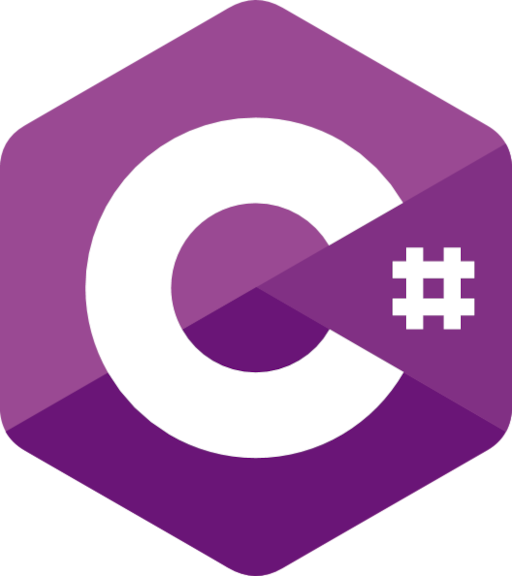
\includegraphics[height=0.12\textwidth]{figures/c.png} & 
C\# es uno de los lenguajes de programación diseñados para la infraestructura de lenguaje común . Su sintaxis básica deriva de C / C++ y utiliza el modelo de objetos de la plataforma .NET, similar al de Java, aunque incluye mejoras derivadas de otros lenguajes.
Para este proyecto en Unity brinda una combinación de eficiencia, integración con el motor de juego y facilidad de aprendizaje, lo que lo convierte en una elección coherente con las necesidades y requisitos del proyecto.
 \\
\hline
\end{tabular}
\caption{Tecnologías}
\end{center}
\end{table}

\clearpage
\subsection{Herramientas de apoyo}
\begin{table}[h!]
\begin{center}
\begin{tabular}{ m{0.15\linewidth} m{0.12\linewidth} m{0.65\linewidth} }
\noalign{\hrule height 2pt}
Nombre & Logo & Descripción \\ 
\noalign{\hrule height 2pt}

Unity & 

\includegraphics[height=0.12\textwidth]{figures/Unity.png} & 
Unity es un motor de desarrollo en tiempo real que te permite crear experiencias interactivas en el Editor de Unity que se utiliza para la creación de videojuegos. Estos se pueden publicar en diversas plataformas como PC, videoconsolas, móviles, etc. Gracias a su flexibilidad es una herramienta que también se usa en diferentes industrias como arquitectura, ingeniería, automotriz y de entretenimiento.
Para este proyecto es una elección sólida debido a su orientación a la creación de simulaciones interactivas, su motor gráfico, la compatibilidad con C#, y su capacidad para facilitar el desarrollo rápido prototipado.
 \\
\hline

Blender & 

\includegraphics[height=0.09\textwidth]{figures/Blender.png} & 
Blender es un programa informático multiplataforma, dedicado especialmente al modelado, iluminación, renderizado, la animación y creación de gráficos tridimensionales. También de composición digital utilizando la técnica procesal de nodos, edición de vídeo, escultura (incluye topología dinámica) y pintura digital.
Para este proyecto puede ser una herramienta valiosa en fases específicas, como la creación detallada de modelos.
\\
\hline

Visual Studio Code & 

\includegraphics[height=0.1\textwidth]{figures/VSC.png} & 
Es un editor de código fuente desarrollado por Microsoft para Windows, Linux y macOS. Incluye soporte para la depuración, control integrado de Git, resaltado de sintaxis, finalización inteligente de código, fragmentos y refactorización de código.
Para este proyecto sería beneficioso, especialmente si se valora un entorno de desarrollo ligero y ágil, una excelente compatibilidad con C# y Unity, y la capacidad de integrar extensiones y herramientas adicionales de manera eficiente
\\ 
\hline

GitHub & 

\includegraphics[height=0.1\textwidth]{figures/GitHub.png} & 
Es un servicio en la nube que ayuda a los desarrolladores a almacenar y administrar su código, al igual que llevar un registro y control de cualquier cambio sobre este código.
Para este proyecto es una herramienta integral para el desarrollo del software y proporciona una infraestructura sólida para la gestión eficiente.

\\ 
\hline

\end{tabular}
\caption{Herramientas de apoyo}
\end{center}
\end{table}
